\documentclass[../IC.tex]{subfiles}

\begin{document}
	\chapter{Hiperbolicidade}
	
	Em geral, na teoria de sistemas dinâmicos, o estudo assintótico de órbitas pode apresentar comportamentos mais robustos, onde pontos fixos e periódicos estão mais espalhados no domínio da dinâmica. Mapas com pontos hiperbólicos são mais comuns, e por isso classificaremos esse pontos neste capítulo.
	
	\begin{definicao}
		Seja $p$ um ponto periódico de período $n$. Chamamos $p$ de hiperbólico se $|(f^n)'(p)| \neq 1$.
	\end{definicao}
	
	\begin{exemplo}
		Considere a função $f(x) = -\dfrac{x^3}{2}-\dfrac{x}{2}$. Temos que $x_1 = 0$ é ponto fixo, enquanto $x_2 = 1, x_3 = -1$ são pontos periódicos de período $2$. Desse modo, temos $f'(x) = -\dfrac{3x^2}{2} - \dfrac{1}{2}$ e $(f^{2})'(x)=\dfrac{\left(\dfrac{3}{4}(x^{3}+x)^{2}+1\right)(3x^{2}+1)}{4}$. Assim, os pontos $x_1,x_2,x_3$ são hiperbólicos, já que
			$$|f'(x_1)| = \dfrac{1}{2}$$
			$$|(f^2)'(x_2)| = 4$$
			$$|(f^2)'(x_3)| = 4.$$
	\end{exemplo}
	
	\begin{definicao}
		Um ponto fixo $p$ é chamado de ponto fixo atrator quando $|f'(p)| < 1$.
	\end{definicao}
	
	\begin{proposicao}
		Considere $p$ um ponto fixo hiperbólico com $|f'(p)| < 1$, onde $f$ é uma função de classe $C^1$. Portanto, existe um intervalo aberto $I$ sobre $p$ de modo que, se $x_0 \in I$, então $$\lim_{n \rightarrow \infty} f^n(x_0) = p.$$
	\end{proposicao}
	
	\begin{prova}
		Como $f$ é de classe $C^1$ e $|f'(p)| < 1$, existe $\epsilon>0$ e $0<A<1$ tal que $|f'(x)|<A, \forall x\in[p-\epsilon, p+\epsilon]$. Seja $x\in[p-\epsilon, p+\epsilon] - \{p\}$. Pelo Teorema do Valor Médio, existe $c$ entre $p$ e $x$ tal que
		$$f'(c) = \frac{f(x)-f(p)}{x-p}=\frac{f(x)-p}{x-p} \implies |f(x)-p|=|f'(c)|\cdot|x-p| \leq A|x-p|<A\cdot\epsilon<\epsilon$$
		Com isso, $f(x) \in [p-\epsilon, p+\epsilon]$ e, usando o mesmo argumento, $|f^2(x)-p|\leq A^2|x-p|<\epsilon$. Continuando dessa maneira, temos $f^n(x)\to p$.
	\end{prova}
	
	\textbf{Observação:} Se $f^n(x)\to p$ quando $n \to \infty$, para cada $x \in I$, seque que o intervalo $I$ está contido na variedade estável $W^s(p)$ de $p$. A proposição anterior também é válida para pontos periódicos hiperbólicos $p$ de período $n$, com $|(f^n)'(p)|<1$.
	
	\begin{definicao}
		Seja $p$ um ponto periódico hiperbólico de período $n$ com $|(f^n)'(p)|<1$. Esse ponto $p$ é chamado de ponto periódico atrator.
	\end{definicao}
	
	\begin{definicao}
		Um ponto fixo $p$ é chamado de ponto fixo repulsor quando $|f'(p)| > 1$.
	\end{definicao}
	
	\begin{proposicao}
		Considere $p$ um ponto fixo hiperbólico com $|f'(p)| > 1$. Assim, existe um intervalo $I$ sobre $p$ de modo que, se $x \in I$, com $x \neq p$, então existe um $k > 0$ tal que $$f^k(x_0) \notin I.$$
	\end{proposicao}
	
	\begin{prova}
		De modo similar ao que foi feito anteriormente, existe $A>1$ tal que se $x \in [p-\epsilon, p+\epsilon]$ então $|f(x)-p|\geq A|x-p|$. Enquanto $f^i(x) \in [p-\epsilon, p+\epsilon]$, teremos $|f^i(x)-p| \geq A^i|x-p|$.
		Como $A>1$, exite $k>0$ tal que $A^k|x-p|>2\epsilon$, isto é, $f^k(x)\notin [p-\epsilon, p+\epsilon]$.
	\end{prova}
	
	\begin{definicao}
		Um ponto fixo $p$ com $|f'(p)|>1$ é chamado de ponto fixo repulsor. A vizinhança descrita na proposição anterior é chama de variedade instável denotada por $W_{loc}^u$.
	\end{definicao}
	
	\textbf{Observação:} Pontos periódicos de período $n$ apresentam comportamento similar ao do ponto fixo repulsor, quando $|(f^n)'(p)| >1$. De modo geral, o comportamento em uma vizinhança de um ponto periódico hiperbólico depende da derivada desse ponto. Isso não ocorre quanto o ponto é não-hiperbólico, como podemos ver no seguinte exemplo.
	
	\begin{exemplo}
		Cada um dos mapas na figura ... satisfaz $f(0) = 0$ e $f'(0)=1$, mas cada um possui um retrato de fase diferente próximo de $0$. em a), o mapa $f(x)=x+x^3$ tem um ponto repulsor em $0$. Em b), o mapa $f(x)=x-x^3$ tem um ponto fixo atrator em $0$. Já em c), o mapa $f(x)=x+x^2$ possui um ponto repulsor à direita mas atrator à esquerda. Um ponto fixo $p$ com $|f'(p)|=1$ é chamado de neutro ou indiferente.
		\begin{center}
		\begin{tikzpicture}[
			line/.style={thick},
			dot/.style={circle, fill=black, inner sep=0pt, minimum size=4pt},
			arrow/.style={->, >={Stealth[length=2.5mm, width=2mm]}, thick}
			]
			
			% ================= ITEM A: Ambos para fora (repulsor) =================
			\begin{scope}[shift={(0, 2.4)}]
				\node[anchor=east] at (-4.2, 0) {\textit{a)}};
				\draw[line] (-4.2, 0) -- (4.2, 0);
				\node[dot] at (0,0) {};
				
				% Esquerda: arcos apontando para a esquerda (<-)
				\draw[arrow] (-0.3, 0) to[out=130, in=50] (-1.5, 0);
				\draw[arrow] (-1.5, 0) to[out=130, in=50] (-3.2, 0);
				
				% Direita: arcos apontando para a direita (->)
				\draw[arrow] (0.3, 0) to[out=50, in=130] (1.5, 0);
				\draw[arrow] (1.5, 0) to[out=50, in=130] (3.2, 0);
			\end{scope}
			
			% ================= ITEM B: Ambos para dentro (atrator) =================
			\begin{scope}[shift={(0, 1.2)}]
				\node[anchor=east] at (-4.2, 0) {\textit{b)}};
				\draw[line] (-4.2, 0) -- (4.2, 0);
				\node[dot] at (0,0) {};
				
				% Esquerda: arcos apontando para a direita (->)
				\draw[arrow] (-3.2, 0) to[out=50, in=130] (-1.5, 0);
				\draw[arrow] (-1.5, 0) to[out=50, in=130] (-0.3, 0);
				
				% Direita: arcos apontando para a esquerda (<-)
				\draw[arrow] (3.2, 0) to[out=130, in=50] (1.5, 0);
				\draw[arrow] (1.5, 0) to[out=130, in=50] (0.3, 0);
			\end{scope}
			
			% ================= ITEM C: Da esquerda para a direita =================
			\begin{scope}[shift={(0, 0)}]
				\node[anchor=east] at (-4.2, 0) {\textit{c)}};
				\draw[line] (-4.2, 0) -- (4.2, 0);
				\node[dot] at (0,0) {};
				
				% Esquerda: arcos apontando para a direita (->)
				\draw[arrow] (-3.2, 0) to[out=50, in=130] (-1.5, 0);
				\draw[arrow] (-1.5, 0) to[out=50, in=130] (-0.3, 0);
				
				% Direita: arcos apontando para a direita (->)
				\draw[arrow] (0.3, 0) to[out=50, in=130] (1.5, 0);
				\draw[arrow] (1.5, 0) to[out=50, in=130] (3.2, 0);
			\end{scope}
			
		\end{tikzpicture}
		\end{center}
	\end{exemplo}
	
	\section{Uma ideia sobre Bifurcação}
	
	Vimos na seção anterior sobre pontos hiperbólicos, que definem atração ou repulsão quando $|f(p)| \neq 1$. Já os pontos não-hiperbólicos trazem um estudo sobre a alteração de comportamento nesses pontos, o que chamamos de bifurcação. Eles ditam uma alteração na dinâmica do sistema, onde pontos periódicos podem surgir ou desaparecer. Alterações no parâmetro da função do sistema causam as mudanças na estrutura.
	
	Consideremos o parâmetro $\mu$ na função $f_\mu(x,\mu)=x+\mu$. Note que a existência de pontos fixos reais na função depende do parâmetro. Existe um determinado valor para $\mu$ tal que o gráfico da função não intersecta mais a reta $y = x$, fazendo com que pontos fixos deixem de existir. Portanto, mesmo uma pequena variação de $\mu$ pode mudar totalmente a estrutura de pontos fixos do sistema.
	\begin{figure}[H]
		\centering
		
\includegraphics[width=0.9\textwidth]{imagens/desenho_familia_quadratica_com_parametro.png}
		\caption{Análise da parábola com parâmetro $\mu$}
	\end{figure}
	Nesta seção, serão estudados dois tipos de bifurcação: Bifurcação de ponto de sela (saddle-node bifurcation) e Bifurcação duplicada de período (period-doubling bifurcation).
	
	A análise de bifurcação de ponto de sela é feita a partir do descobrimento de pontos da função, onde há a classificação dos mesmos. Já na bifurcação duplicada de período, essa mesma análise agora é feita nas iterações da função, sendo que nesse caso os pontos analisados agora serão os pontos periódicos.
	
	\begin{exemplo}\label{primeiroExemploBifurcacao}
		Tomemos o sistema dinâmico $(\mathbb{R}, f)$, onde $f_\mu(x,\mu)=x+\mu$ com sua derivada dada por $f_\mu'(x)=2x$. Logo, os pontos fixos da função são aqueles que satisfazem $x^2+\mu=x$. Por Bháskara, temos que esses pontos são
		$$x_1 = \dfrac{1+\sqrt{1-4\mu}}{2}, x_2 = \dfrac{1-\sqrt{1-4\mu}}{2}$$
		Como $f: \mathbb{R} \rightarrow \mathbb{R}$, precisamos garantir $\mu$ tal que a raiz seja real. $1-4\mu \geq 0 \implies \mu \leq \dfrac{1}{4}$.
		\begin{itemize}
			\item $\mu > \dfrac{1}{4}$: 
			
			Resulta $x_1$ e $x_2$ como pontos fixos complexos, o que significa que o gráfico da função está acima da reta $y=x$. Desse modo, consideramos que não existem pontos fixos.
			\item $\mu = \dfrac{1}{4}$:
			
			Temos que $x_1 = x_2 = \dfrac{1}{2}$, portanto, um ponto fixo apenas.
			\begin{figure}[H]
				\centering
				
\includegraphics[width=0.3\textwidth]{imagens/desenho_quadratica_1-4.png}
				\caption{Análise da parábola com parâmetro $\mu = \dfrac{1}{4}$}
			\end{figure}
			Para o ponto fixo $x=\dfrac{1}{2}$, temos que ele é não-hiperbólico (ponto de sela), pois $f_\mu'\left(\dfrac{1}{2}\right)=1$. Logo, temos uma bifurcação nesse ponto.
			
			A partir do mapeamento do ponto fixo, é possível definir seu conjunto estável, dado pelos valores de $x$ que convergem para $\dfrac{1}{2}$. Também é possível analisar o conjunto instável, onde essa análise se dá na função inversa.
			\begin{figure}[H]
				\centering
				
\includegraphics[width=0.6\textwidth]{imagens/desenho_conjunto_estavel_1-4.jpg}
				\caption{Análise de estabilidade do ponto fixo $x = \dfrac{1}{2}$}
			\end{figure}
			Pelo retrato de fases, é possível concluir que o conjunto estável de $\dfrac{1}{2}$, ou seja, aqueles pontos em que $f^i(x) \rightarrow \dfrac{1}{2}, i \rightarrow \infty$  é dado por $W^s(\frac{1}{2}) = \{x \in \mathbb{R} : -\frac{1}{2} \leq x \leq \frac{1}{2}\}$. Isso significa que qualquer ponto fora do intervalo tem órbita convergindo para $\infty$.
			
			Já o conjunto instável, sob análise da função inversa, é facilmente descrito pelo seu gráfico usando o mesmo processo de retrato de fases.
			
			\begin{figure}[H]
				\centering
				
\includegraphics[width=0.6\textwidth]{imagens/desenho_conjunto_instavel_1-4.png}
				\caption{Análise de instabilidade do ponto fixo $x = \dfrac{1}{2}$}
			\end{figure}
			
			Temos que qualquer ponto no intervalo $-\frac{1}{2} < x < \frac{1}{2}$ não tem órbita convergindo para o ponto fixo. Já fora desse intervalo, os pontos convergem para o ponto fixo após $f^i(x)$, com $i \rightarrow \infty$. Portanto, definimos o conjunto instável por $W^u(\frac{1}{2}) = (-\infty, -\frac{1}{2}] \cup [\frac{1}{2}, \infty)$.
			\item $\mu < \dfrac{1}{4}$:
			
			Resulta que o gráfico da função passa a intersectar a reta $y=x$ em dois pontos, isto é, $x_1 \neq x_2$.			
			
			Note que a alteração no parâmetro $\mu$ leva a função de nenhum ponto fixo para dois pontos fixos.
			
			Agora podemos classificar $x_1$ e $x_2$ como atratores ou repulsores quando $\mu < \dfrac{1}{4}$. Para que $x_1$ seja repulsor, deve existir $\mu$ tal que $|f_\mu'(x_1)| > 1$.
			$$\left|2\left(\dfrac{1+\sqrt{1-4\mu}}{2}\right)\right| > 1 \implies |1+\sqrt{1-4\mu}| > 1 \implies \sqrt{1-4\mu} > 0 \implies \mu < \dfrac{1}{4}$$ Logo, $x_1$ é repulsor $\forall\mu < \dfrac{1}{4}$. 
			
			Para que $x_2$ seja atrator, deve existir $\mu$ tal que $|f_\mu'(x_2)| < 1$, ou seja, $-1 < f_\mu'(x_2) < 1$.
			$$-1 < 2\left(\dfrac{1-\sqrt{1-4\mu}}{2}\right) < 1 \implies -1 < 1-\sqrt{1-4\mu} < 1 \implies -2 < -\sqrt{1-4\mu} < 0$$
			$$ \implies 4 > 1-4\mu > 0 \implies 3>-4\mu>-1 \implies -\dfrac{3}{4}<\mu<\dfrac{1}{4}$$ Logo, $x_2$ é atrator quando $-\dfrac{3}{4}<\mu<\dfrac{1}{4}$.
			
			Com isso, a definição do conjunto estável dos dois pontos fixos pode ser observada de forma genérica no intervalo de $\mu$, através do retrato de fases feito no próprio gráfico da função. 
			
			Desse modo, definimos o conjunto $W^s(x_1)$ como $W^s(x_1) = \{-x_1, x_1\}$, pois qualquer outro ponto faz valer o que definimos há pouco: $x_1$ é um ponto fixo repulsor, fazendo com que a órbita se afaste dele. 
			
			Já para $x_2$, que vimos ser um ponto atrator, temos $W^s(x_2) = \{x \in \mathbb{R} : -x_1 < x < x_1\}$. Isso significa que para qualquer $x \in (-x_1, x_1)$, $f^i(x) \rightarrow x_2$, com $i \rightarrow \infty$.
			
			\begin{figure}[H]
				\centering
				
\includegraphics[width=0.8\textwidth]{imagens/desenho_conjunto_estavel_dois_pontos.png}
				\caption{Análise de estabilidade dos pontos fixos $x_1$ e $x_2$}
			\end{figure}
			
			Já vimos que para $\mu = \dfrac{1}{4}$, temos um ponto fixo não-hiperbólico, indicando uma bifurcação. O mesmo acontece para $\mu = -\dfrac{3}{4}$, indicando uma nova bifurcação acontecendo em $x_2$.
			
			No entanto, quando $\mu < -\dfrac{3}{4}$, acontece uma mudança em $x_2$. Ao analisar $|f_\mu'(x)|$, temos
			$$\left|2\left(\dfrac{1-\sqrt{1-4\mu}}{2}\right)\right| \implies |1-\sqrt{1-4\mu}|$$
			A raiz quadrada nos mostra que $\sqrt{1-4\mu} > 2$, pois $-4\mu > 3$. Portanto, $x_2$ passa a ser repulsor, já que $|1-\sqrt{1-4\mu}| > 1, \forall \mu<-\dfrac{3}{4}$.
		\end{itemize}
	\end{exemplo}
	
	\begin{exemplo}
		Considerando ainda o mesmo cenário do Exemplo $\ref{primeiroExemploBifurcacao}$, agora analisando a segunda iterada da função, ou seja, $f_\mu^2(x, \mu) = x^4 + 2x^2\mu+\mu^2+\mu$, com derivada dada por $(f_\mu^2)'(x,\mu)=4x^2+4x\mu$, temos o surgimento de pontos periódicos de período $2$ para análise.
		
		\noindent Temos como pontos fixos de $f_\mu^2$ os pontos que satisfazem a equação $x^4 + 2x^2\mu+\mu^2+\mu = x$. Para facilitar a identificação desses pontos, vamos tomar essa mesma equação fatorada: $$(\underbrace{x^2+\mu-x}_{(I)})(\underbrace{x^2-\mu+x+1}_{(II)})=0$$
		\noindent A equação fatorada é dada pelo produto de duas quadráticas, onde as soluções de cada uma são os pontos que estamos procurando. Note que o fator (I) é justamente a solução dos pontos fixos do Exemplo $\ref{primeiroExemploBifurcacao}$, o que faz sentido, já que são os pontos que aparecem em todas as iteradas. Agora, além dos pontos fixos, temos a aparição de pontos periódicos em (II) que também são soluções da equação, e são esses pontos que iremos analisar. Logo, as soluções da equação (II) (pontos periódicos), por Bháskara, são
		$$x_1=\dfrac{-1+\sqrt{-4\mu-3}}{2},x_2=\dfrac{-1-\sqrt{-4\mu-3}}{2}$$
		Novamente, como $f: \mathbb{R} \rightarrow \mathbb{R}$, temos que garantir $\mu$ tal que $-4\mu-3\geq0$. Logo, 
		$$-4\mu-3\geq0 \implies \mu \leq -\dfrac{3}{4}$$
		
		\begin{itemize}
			\item $\mu > -\dfrac{3}{4}$:
			
			Resulta $x_1$ e $x_2$ como pontos periódicos em $\mathbb{C}$, portanto saem do escopo de estudo em $\mathbb{R}$.			
			\item $\mu = -\dfrac{3}{4}$:
			
			Temos que $x_1 = x_2 = -\dfrac{1}{2}$, portanto, um ponto periódico apenas. Para esse ponto, temos que sua classificação é de ponto de sela, indicando bifurcação, pois $\left|(f_\mu^2)'\left(-\dfrac{1}{2}, -\dfrac{3}{4}\right)\right| = 1$.
			
			\item $\mu < -\dfrac{3}{4}$:
			
			Temos que $(f_\mu^2)'(x_1, \mu) = 4+4\mu$. Para classificarmos $x_1$ como atrator, precisamos garantir $\mu$ tal que $|4+4\mu| < 1$, ou seja, $-1 < 4+4\mu < 1$. Logo, 
			$$-1 < 4+4\mu < 1 \implies -5 < 4\mu < -3 \implies -\dfrac{5}{4} < \mu < -\dfrac{3}{4}$$
			Portanto, $x_1$ é atrator quando $-\dfrac{5}{4} < \mu < -\dfrac{3}{4}$.
			Para $x_2$, temos que $(f_\mu^2)'(x_2, \mu) = 4+4\mu$, ou seja, temos o mesmo caso de $x_1$, fazendo com que $x_2$ também seja atrator quando $\mu \in \left(-\dfrac{5}{4},-\dfrac{3}{4}\right)$.
			
			Note que quando chegamos na fronteira $-\dfrac{5}{4}$ do intervalo, a classificação de $x_1$ e $x_2$ passa a ser de pontos de sela, já que 
			$\left|(f_\mu^2)'\left(x_1, -\dfrac{5}{4}\right)\right| = \left|(f_\mu^2)'\left(x_2, -\dfrac{5}{4}\right)\right| = 1$. Assim, temos novas bifurcações acontecendo simultaneamente tanto em $x_1$ quanto em $x_2$ para $\mu = -\dfrac{5}{4}$, e nesse caso, a continuidade do estudo dessas novas bifurcações se dá em $f_\mu^3(x, \mu)$.
			
		\end{itemize}
		O gráfico abaixo mostra visualmente o que foi analisado sobre os pontos neste exemplo e no Exemplo $\ref{primeiroExemploBifurcacao}$.
		\begin{center}
			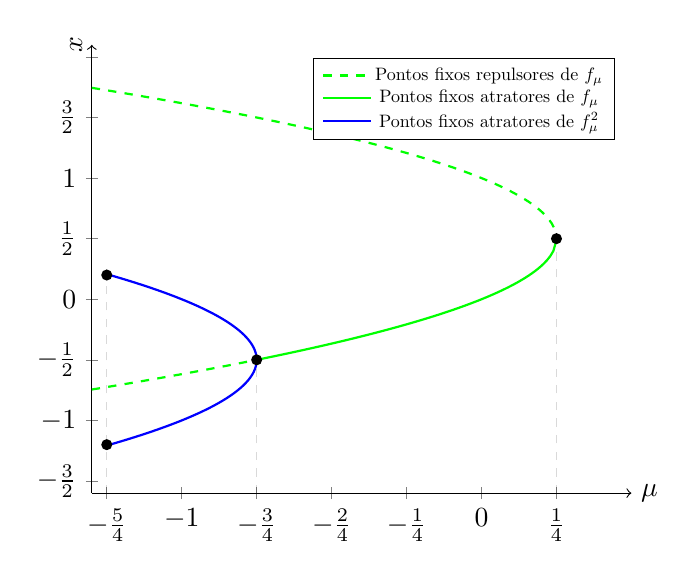
\begin{tikzpicture}
				\begin{axis}[
					axis lines = left,
					xlabel = {$\mu$},
					ylabel = {$x$},
					xmin = -1.3, xmax = 0.5,
					ymin = -1.6, ymax = 2.1,
					xtick={-1.25, -1, -0.75, -0.5, -0.25, 0, 0.25},
					xticklabels={$-\frac{5}{4}$, $-1$, $-\frac{3}{4}$, $-\frac{2}{4}$, $-\frac{1}{4}$, $0$, $\frac{1}{4}$},
					ytick={-1.5, -1, -0.5, 0, 0.5, 1, 1.5, 2},
					yticklabels={$-\frac{3}{2}$, $-1$, $-\frac{1}{2}$, $0$, $\frac{1}{2}$, $1$, $\frac{3}{2}$},
					y label style={at={(0,1)},above},
					x label style={at={(1,0)},right},
					axis line style={->},
					legend pos = north east,
					legend style={nodes={scale=0.65, transform shape}}
					]
					
					\addplot [domain=-1.3:0.25, samples=200, thick, green, dashed] 
					{0.5 + 0.5*sqrt(1 - 4*x)};   
					\addlegendentry{Pontos fixos repulsores de $f_\mu$}
					
					\addplot [domain=-0.75:0.25, samples=100, green, thick] 
					{0.5 - 0.5*sqrt(1 - 4*x)};
					\addlegendentry{Pontos fixos atratores de $f_\mu$}
					
					\addplot [domain=-1.3:-0.75, samples=100, green, thick, dashed, forget plot] 
					{0.5 - 0.5*sqrt(1 - 4*x)};
					
					\addplot [domain=-1.25:-0.75, samples=200, blue, thick] 
					{-0.5 + 0.5*sqrt(-4*x - 3)};
					\addlegendentry{Pontos fixos atratores de $f_\mu^2$}
					
					\addplot [domain=-1.25:-0.75, samples=200, blue, thick, forget plot] 
					{-0.5 - 0.5*sqrt(-4*x - 3)};
					
					\fill (axis cs:0.25,0.5) circle (2pt);
					\fill (axis cs:-0.75,-0.5) circle (2pt);
					\fill (axis cs:-1.25,-1.2) circle (2pt);
					\fill (axis cs:-1.25,0.2) circle (2pt);
					
					\addplot [black, dashed, forget plot, opacity=0.15] coordinates {(-0.75, -1.6) (-0.75, -0.5)};
					\addplot [black, dashed, forget plot, opacity=0.15] coordinates {(0.25, -1.6) (0.25, 0.5)};
					\addplot [black, dashed, forget plot, opacity=0.15] coordinates {(-1.25, -1.6) (-1.25, 0.25)};
					
				\end{axis}
			\end{tikzpicture}
			\captionof{figure}{Bifurcação}
		\end{center}
	\end{exemplo}
\end{document}